\documentclass{article}
\usepackage[utf8]{inputenc}
\usepackage{amsmath}
\usepackage{graphicx}
\usepackage{physics}
\begin{document}
\section{Problem 2 within project 1}


\begin{figure}
    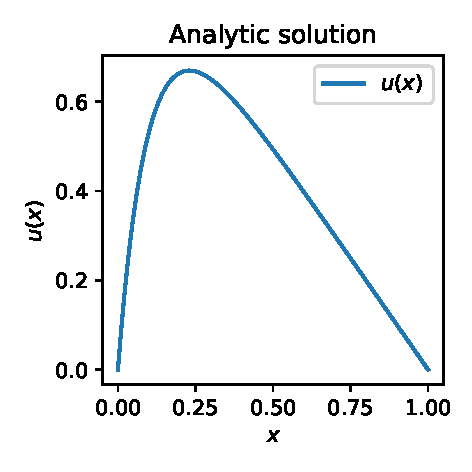
\includegraphics{problem_2_fig.pdf}
    \caption{Shows 100 linearly spaced points between 0 and 1, evaluated on the excact solution $u(x)=1 - (1 - e^{-10})x - e^{-10x}$.}
\end{figure}


\end{document}